\section{Introduction}

Data visualisation is essential to data science and science communication. Its
power as a communicative tool means it is also open to misinterpretation and
misuse: patterns in raw data can be obscured, statistical assumptions hidden,
and effect sizes misrepresented \cite{weissgerber15}. These concerns can be
addressed in part through improved statistical practices and novel plot and
chart designs \cite{allen19}, but also by making visualisations themselves more
open and explorable \cite{dragicevic19}.

An important aspect of explorability that has been studied for several decades
are techniques for helping the user grasp how a visualisation relates to other
concurrent visualisations of the same underlying data. For example,
geoscientists often work with multiple layered views. To show how these are
related, spatial analytics applications like GeoDa \cite{anselin06} can
automatically select the relevant part of one view as the user changes the
selection in a related view, say a choropleth map. However, this feature is
available only if it was specifically anticipated by the application or library
developer; if the geoscientist uses custom libraries or wants other views linked
that the developer did not onsider, they are out of luck.

\begin{figure}[H]
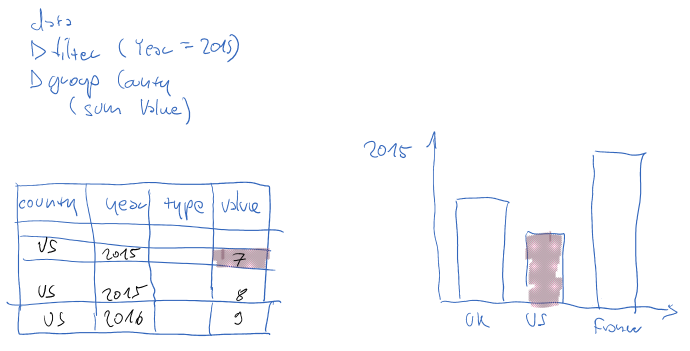
\includegraphics[scale=0.35]{image/chart-fwd}
\caption{Forward linking from code and data to visualisation}
\end{figure}

In this paper we present a framework for authoring visualisations where support
for linking, between data, code, and visualisations is built in, making this
powerful comprehension feature automatic.

\cite{becker87,buja91}

\section{Another section}

Our framework provides infrastructure for ``linking'', or multiple-coordinated
views \cite{tobiasz09}, in an application-independent way. The theoretical
foundation of the work is our own prior work on dynamic dependency analysis and
provenance \cite{perera16d, ricciotti17}; in contrast to prior work on
provenance in data visualisation \cite{callahan06}, our approach is much more
fine-grained and is able to associate specific parts of the data or code with
parts of a visualisation in a precise way. While the theoretical technique is
proven, this approach has never been applied to data visualisation before.

\begin{figure}[H]
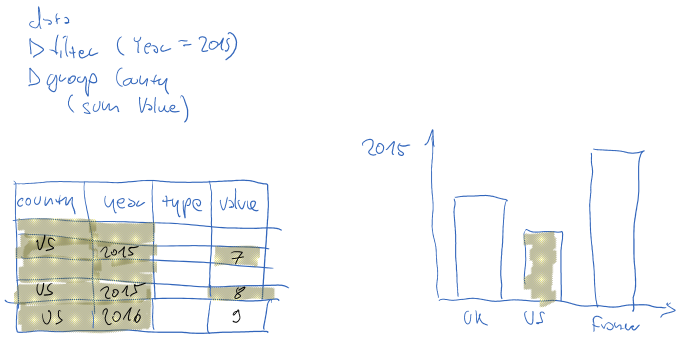
\includegraphics[scale=0.35]{image/chart-bwd}
\caption{Backward linking from visualisation to code and data}
\end{figure}

\section{Conclusions and future work}

There are a number of challenges associated with making our approach practical
and appealing to actual data scientists. A central usability challenge is
visualising these complex relationships between the various parts of a
visualisation and the relevant data and/or visualisation code. This is
essentially a higher-order visualisation problem: visualising information about
the provenance of visualisations. Ideas from temporal data visualisation
\cite{bach16}, data-driven storytelling \cite{bach18}, and ``literate''
visualisation \cite{wood19} may inform our efforts here.
